\documentclass[12pt]{article}
\usepackage{fullpage}
\usepackage{graphicx}
\usepackage{amsfonts}
\usepackage{color}
\usepackage{soul}
\pagestyle{plain}
\setlength{\oddsidemargin}{0.5in}
\setlength{\evensidemargin}{0.5in}
\setlength{\textwidth}{6.0in}
\renewcommand{\baselinestretch}{1.2}
\newcommand{\Dsl}{{\not\!\! D}}
\newcommand{\psl}{{\not\! p}}
\usepackage{gensymb}
\usepackage{tikzsymbols}
\usepackage[utf8]{inputenc}
\usepackage{array}
\usepackage{makecell}
\usepackage{hyperref}

\renewcommand\theadalign{bc}
\renewcommand\theadfont{\bfseries}
\renewcommand\theadgape{\Gape[4pt]}
\renewcommand\cellgape{\Gape[4pt]}

%Above are the packages that are needed for most of the reports that you will write
%%%%%%%%%%%%%%%%%%%%%%%%%%%%%%%%%%%%%%%%%%%


\title{Is Reaction Time Important?}
\author{Kody Rogers}
\date{\today}
\begin{document}

\maketitle
\thispagestyle{empty}

%Above is title stuff
%%%%%%%%%%%%%%%%%%%%%%%%%%%%%%%%%%%%%%%%%%%%%
\section{The Dilema}
Some people say that a goaltender needs to have a quick reaction time to succeed in hockey. I read once that reaction time is actually not that important, because the shots that goaltenders have to stop are usually moving too fast to react to. How about lets go through a couple of examples to see if this is true.

\section{Top Corner From the Blue Line}
Let's say a player is facing the net and decides to go top corner from the blue line. The distance from the blue line to the goal line is 64 ft and the height of the net is 4ft. If the puck is shot at 80mph (v = 80 mph) how much time does the goalie have to react to the shot? Is it possible for any human to react that fast?

\begin{figure}[h]
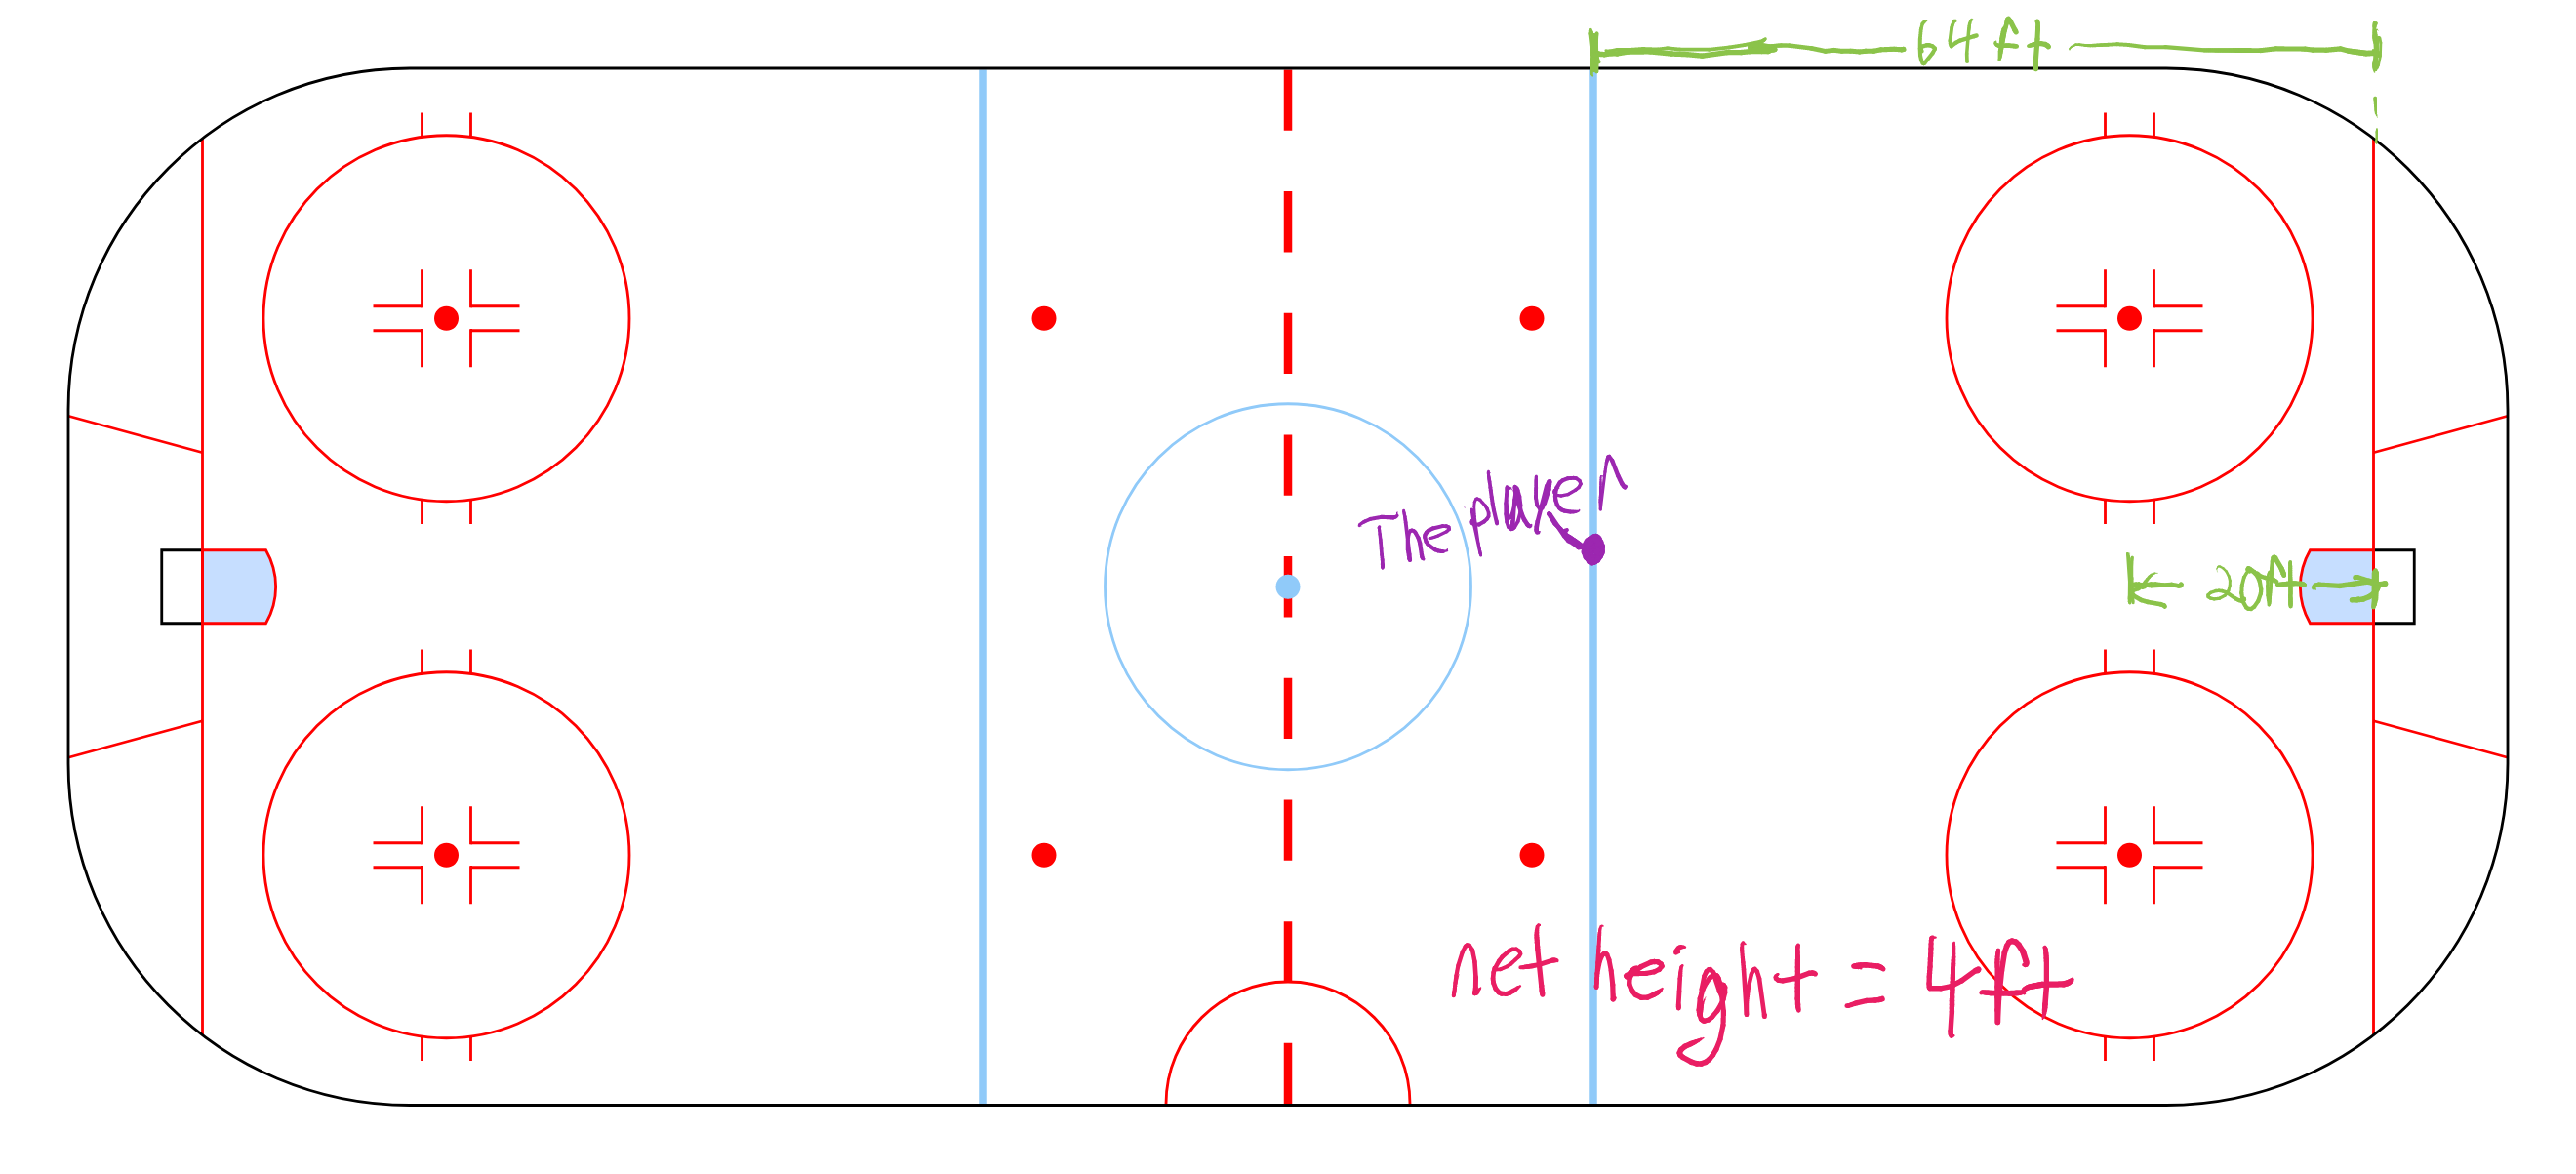
\includegraphics[scale=0.15]{OutlineForHockeyWorksheet.png}
\end{figure}


\subsection{Convert to Acceptable Units}
It may be a good idea to first convert the units from ft and mph into something more familiar. I am from Saskatchewan and at our schools we tend to use $\frac{m}{s}$ or $\frac{km}{hour}$ for speed and $m$ for distance. Use the space below to convert to whatever units you feel most comfortable with.

\parbox[][8cm][t]{8cm}{}

\subsection{Calculate Total Distance Traveled}
The next step to take is to calculate the total distance that the puck needs to travel. To do this constructing a triangle with the dimensions from the start (4ft height 64ft long) and then solve for the hypotaneus. Use the space below to create a diagram of the triangle.

\parbox[][7cm][t]{8cm}{}

Now use your knowledge of trigonometry (mostly pythagarean theorem) to calculate the hypotaneus.

\parbox[][8cm][t]{8cm}{}

\subsection{Final Calculation}
Now using the following equation, $d = vt$ it should be possible to solve for the time it takes to hit the net. Does this leave enough time for the goalie to react? Look up the average reaction time for a human, and then think about whether or not a goalie would be able to move fast enough to stop the shot without anticipating what the player was going to do.

\parbox[][8cm][t]{8cm}{}

\section{Top Corner from the slot}
Now, using the same diagram, calculate the time it takes a shot taken from the slot to reach the net. The slot is 20 ft from the net, and the net is the same height. Do both the top shelf calculations and the calculation if the puck stays on the ice.

\parbox[][16cm][t]{12cm}{}

\begin{flushleft}
    \copyright  2020 Kody Rogers - kodyrogers21@gmail.com.

    This work is is licensed under a Creative Commons Attribution 4.0 International License.

    \url{https://creativecommons.org/licenses/by/4.0/}.
\end{flushleft}

%Above is the Discussion
%%%%%%%%%%%%%%%%%%%%%%%%%%%%%%%%%%%%%%%%%%%%%%%%%%%%%%%
\end{document}
